\documentclass[11pt,]{article}
\usepackage[left=1in,top=1in,right=1in,bottom=1in]{geometry}
\newcommand*{\authorfont}{\fontfamily{phv}\selectfont}
\usepackage[]{mathpazo}


  \usepackage[T1]{fontenc}
  \usepackage[utf8]{inputenc}



\usepackage{abstract}
\renewcommand{\abstractname}{}    % clear the title
\renewcommand{\absnamepos}{empty} % originally center

\renewenvironment{abstract}
 {{%
    \setlength{\leftmargin}{0mm}
    \setlength{\rightmargin}{\leftmargin}%
  }%
  \relax}
 {\endlist}

\makeatletter
\def\@maketitle{%
  \newpage
%  \null
%  \vskip 2em%
%  \begin{center}%
  \let \footnote \thanks
    {\fontsize{18}{20}\selectfont\raggedright  \setlength{\parindent}{0pt} \@title \par}%
}
%\fi
\makeatother




\setcounter{secnumdepth}{3}

\usepackage{longtable,booktabs}

\usepackage{graphicx,grffile}
\makeatletter
\def\maxwidth{\ifdim\Gin@nat@width>\linewidth\linewidth\else\Gin@nat@width\fi}
\def\maxheight{\ifdim\Gin@nat@height>\textheight\textheight\else\Gin@nat@height\fi}
\makeatother
% Scale images if necessary, so that they will not overflow the page
% margins by default, and it is still possible to overwrite the defaults
% using explicit options in \includegraphics[width, height, ...]{}
\setkeys{Gin}{width=\maxwidth,height=\maxheight,keepaspectratio}

\title{Ecología numérica de la familia Myrtaceae en la parcela permanente de
50-ha en Barro Colorado, lago Gatún, Panamá\\
Subtítulo\\
Subtítulo  }



\author{\Large Rosee Aurelina Féliz Méndez\vspace{0.05in} \newline\normalsize\emph{Estudiante, Universidad Autónoma de Santo Domingo (UASD)}  }


\date{}

\usepackage{titlesec}

\titleformat*{\section}{\normalsize\bfseries}
\titleformat*{\subsection}{\normalsize\itshape}
\titleformat*{\subsubsection}{\normalsize\itshape}
\titleformat*{\paragraph}{\normalsize\itshape}
\titleformat*{\subparagraph}{\normalsize\itshape}

\titlespacing{\section}
{0pt}{36pt}{0pt}
\titlespacing{\subsection}
{0pt}{36pt}{0pt}
\titlespacing{\subsubsection}
{0pt}{36pt}{0pt}





\newtheorem{hypothesis}{Hypothesis}
\usepackage{setspace}

\makeatletter
\@ifpackageloaded{hyperref}{}{%
\ifxetex
  \PassOptionsToPackage{hyphens}{url}\usepackage[setpagesize=false, % page size defined by xetex
              unicode=false, % unicode breaks when used with xetex
              xetex]{hyperref}
\else
  \PassOptionsToPackage{hyphens}{url}\usepackage[unicode=true]{hyperref}
\fi
}

\@ifpackageloaded{color}{
    \PassOptionsToPackage{usenames,dvipsnames}{color}
}{%
    \usepackage[usenames,dvipsnames]{color}
}
\makeatother
\hypersetup{breaklinks=true,
            bookmarks=true,
            pdfauthor={Rosee Aurelina Féliz Méndez (Estudiante, Universidad Autónoma de Santo Domingo (UASD))},
             pdfkeywords = {Myrtaceae, Ecología numérica},  
            pdftitle={Ecología numérica de la familia Myrtaceae en la parcela permanente de
50-ha en Barro Colorado, lago Gatún, Panamá\\
Subtítulo\\
Subtítulo},
            colorlinks=true,
            citecolor=blue,
            urlcolor=blue,
            linkcolor=magenta,
            pdfborder={0 0 0}}
\urlstyle{same}  % don't use monospace font for urls

% set default figure placement to htbp
\makeatletter
\def\fps@figure{htbp}
\makeatother

\usepackage{pdflscape} \newcommand{\blandscape}{\begin{landscape}}
\newcommand{\elandscape}{\end{landscape}}


% add tightlist ----------
\providecommand{\tightlist}{%
\setlength{\itemsep}{0pt}\setlength{\parskip}{0pt}}

\begin{document}
	
% \pagenumbering{arabic}% resets `page` counter to 1 
%
% \maketitle

{% \usefont{T1}{pnc}{m}{n}
\setlength{\parindent}{0pt}
\thispagestyle{plain}
{\fontsize{18}{20}\selectfont\raggedright 
\maketitle  % title \par  

}

{
   \vskip 13.5pt\relax \normalsize\fontsize{11}{12} 
\textbf{\authorfont Rosee Aurelina Féliz Méndez} \hskip 15pt \emph{\small Estudiante, Universidad Autónoma de Santo Domingo (UASD)}   

}

}








\begin{abstract}

    \hbox{\vrule height .2pt width 39.14pc}

    \vskip 8.5pt % \small 

\noindent Resumen del manuscrito


\vskip 8.5pt \noindent \emph{Keywords}: Myrtaceae, Ecología numérica \par

    \hbox{\vrule height .2pt width 39.14pc}



\end{abstract}


\vskip 6.5pt


\noindent  \section{Introducción}\label{introducciuxf3n}

La isla de Barro Colorado (BCI, por sus siglas en inglés) se formó al
término del canal de Panamá en 1974, desde su creación se ha utilizado
como centro de investigación debido a su reserva natural. Se considera
monumento natural protegido por el gobierno de Panamá junto a las
penínsulas Peña Blanca, Bohío, Buena Vista, Frijoles y Gigante. La
parcela permanente de 50 hectáreas se encuentra en el bosque húmedo
tropical de la isla de Barro Colorado. Se estableció en 1980, desde
entonces se han realizado 8 censos (aprox. 1 cada 5 años) en cual se
toman en cuenta arboles de tallos leñosos con un diámetro a la altura
del pecho (DAP) mayor a 10 mm, y como resultado en cada censo, se han
identificado, censado y mapeado más de 350, 000 árboles individuales.

Se ha seleccionado el censo número 8 de esta reserva natural por ser el
más reciente y a esta reserva natural en particular debido a la gran
cantidad disponible de datos censales que a través de la Ecología
numérica nos permitirán conocer rasgos básicos de la estructura y
composición de la comunidad de plantas mirtáceas en relación con
factores ambientales.

Familia Myrtaceae

R

En este trabajo se harán estudios de asociación, agrupamiento,
diversidad y ecología espacial en relación a factores ambientales con
los datos disponibles del censo número de 8 de la parcela permanente de
50-ha con ecología numérica en R para comprender mejor la estructura y
composición de la comunidad de mirtáceas en la foresta tropical de Barro
Colorado.

\section{Metodología}\label{metodologuxeda}

\ldots

\section{Resultados}\label{resultados}

La tabla \ref{tab:abun_sp} y la figura \ref{fig:abun_sp_q} visualiza
estos resultados a continuación.

\begin{longtable}[]{@{}lr@{}}
\caption{\label{tab:abun_sp}Abundancia por especie de la familia
Myrtaceae}\tabularnewline
\toprule
Latin & n\tabularnewline
\midrule
\endfirsthead
\toprule
Latin & n\tabularnewline
\midrule
\endhead
Eugenia galalonensis & 1975\tabularnewline
Eugenia oerstediana & 1838\tabularnewline
Eugenia coloradoensis & 609\tabularnewline
Chamguava schippii & 541\tabularnewline
Eugenia nesiotica & 502\tabularnewline
Psidium friedrichsthalianum & 58\tabularnewline
Myrcia gatunensis & 56\tabularnewline
\bottomrule
\end{longtable}

\begin{figure}
\centering
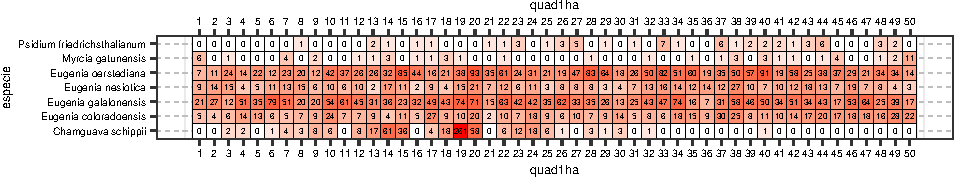
\includegraphics{manuscrito_files/figure-latex/unnamed-chunk-3-1.pdf}
\caption{\label{fig:abun_sp_q}Abundancia de especies por quadrat}
\end{figure}

\section{Discusión}\label{discusiuxf3n}

\section{Agradecimientos}\label{agradecimientos}

\section{Información de soporte}\label{informaciuxf3n-de-soporte}

\ldots

\section{\texorpdfstring{\emph{Script}
reproducible}{Script reproducible}}\label{script-reproducible}

\ldots

\section{Referencias}\label{referencias}




\newpage
\singlespacing 
\end{document}
